\documentclass[a4paper, AutoFakeBold=2.17 ,zihao=-4]{ctexart}

\usepackage[margin=1in]{geometry}

\usepackage{amsmath,amssymb,amsthm}
\usepackage{newtxmath}
\usepackage{fancyhdr}
\usepackage{fontspec}
\usepackage{booktabs}
\usepackage{xeCJKfntef}
\usepackage{titling}
\usepackage{subcaption}
\usepackage{listings}
\usepackage{float}
\usepackage[export]{adjustbox}
\usepackage{caption}
\usepackage{enumerate}
\usepackage{xcolor}
\usepackage{diagbox}
\usepackage{mathrsfs}
\usepackage{appendix}
\usepackage{svg}
\usepackage{tabularx}
\usepackage{tabularray}
\usepackage{multirow}
\usepackage{zhlipsum}
\usepackage{siunitx}
\usepackage{tikz}
\usepackage{graphicx}
\usepackage{eso-pic}
\usepackage{pagecolor}
\usepackage{minted}
\usepackage{hyperref}
\usepackage{pgffor}
\usepackage{enumitem}
\usepackage{pifont}
\usepackage{multicol}


\ctexset{
    section={
        format=\zihao{4}\bfseries\heiti,
        name={,、},
        number=\chinese{section}
    },
    subsection={
        format=\bfseries\heiti,
    }
}

\graphicspath{{./figures/}}
\svgpath{{./figures/}}
\DeclareGraphicsExtensions{.pdf, .jpg, .png}

\renewcommand\maketitlehooka{\null\mbox{}\vfill}
\renewcommand\maketitlehookd{\vfill\null}

\title{
    \centering{
\includegraphics[width=.8\columnwidth]{LOGO_light}}\\
    \vfill
    \begin{tblr}{
                   hlines,
                   stretch = 2,
                   width = \columnwidth,
                   cells ={c,m}
               }
    \Huge\bfseries\heiti“高级语言程序设计”课程设计项目报告
    \end{tblr}
}
\author{
    \Large\texttt{Jesse Senior}
    \and
    \Large\texttt{Xshellye}
}

\date{}

\newcommand\BackgroundPicture{%
    \put(0,0){%
        \parbox[b][\paperheight]{\paperwidth}{%
            \vfill
            \centering%
        \begin{tikzpicture}[remember picture,overlay]
        \node [rotate=57.1,scale=1,text opacity=0.1] at (current page.center) {
\includegraphics{icon}};
        \end{tikzpicture}%
        \vfill
        }
    }
}

\UseTblrLibrary{booktabs} 

\newlist{todolist}{itemize}{2}
\setlist[todolist]{label=$\square$}
\newcommand{\cmark}{\ding{51}}%
\newcommand{\xmark}{\ding{55}}%
\newcommand{\done}{\rlap{$\square$}{\raisebox{2pt}{\large\hspace{1pt}\cmark}}%
\hspace{-2.5pt}}
\newcommand{\wontfix}{\rlap{$\square$}{\large\hspace{1pt}\xmark}}

%%%%%%%%%%%%%%%%%%%%%%%

\begin{document}

\AddToShipoutPicture{\BackgroundPicture}
\maketitle
\thispagestyle{empty}
\setcounter{page}{0}
\tikz[overlay]\path[opacity=0.1](0,0);
\clearpage
\ClearShipoutPicture

\section{项目目标}

应用面向对象编程的相关知识,设计一个简单五子棋游戏。

\paragraph{具体要求:}
\begin{enumerate}
    \item 实现五子棋人人对战、人机对战;
    \item 支持对战历史记录显示、复盘、删除,支持对战信息统计;
    \item 充分应用面向对象思维,合理应用类、对象、封装、继承、多态等特性,\\
          其中:
          \begin{enumerate}
              \item 类的数量应不少于5;
              \item 继承层次结构的数量应不少于2;
          \end{enumerate}
    \item 界面设计精美,交互设计友好;
    \item 支持随机文件处理(读、写、改);
    \item 源代码总行数不少于2000。
\end{enumerate}

\section{项目设计}

\subsection{前期分析}

考虑到五子棋人机对战存在应用神经网络算法的可能,以及语言对于功能的封装程度、编译环境搭建难度、跨平台性等各种因素,由于C++自身封装程度低,需要自己“重新发明轮子”(如OpenGL),且使用第三方库过程复杂、开发过程中容易增加沟通阻碍(如OpenCV),因此本项目并未选择使用C++作为项目开发语言,而最终决定选择封装程度高、开发难度相对更小的python作为项目开发语言。

在此基础上,考虑到游戏相对于其他软件的特殊性,最终选择封装相对底层、自由度更高的pygame作为项目GUI渲染引擎,并按照项目实际需要对其重新进行封装。

由于项目涉及到对战历史记录的存储,考虑到数据自身结构性强,增删改查规范,最终选择轻量化本地数据库SQLite以支持高稳定性的随机文件读写。

\subsection{总体设计}

\subsubsection{系统组成}

根据项目目标,我们将项目划分为四个主要模块:

\begin{table}[H]
    \centering
    \begin{tblr}{
            width = .6\columnwidth,
            cells ={l,m}
        }
        \toprule
        模块名    & 项目路径                     \\
        \midrule
        核心逻辑模块 & \texttt{src/core.py}     \\
        数据库模块  & \texttt{src/database.py} \\
        AI模块   & \texttt{src/ai.py}       \\
        GUI模块  & \texttt{src/display/}    \\
        \bottomrule
    \end{tblr}
\end{table}

\begin{description}
    \item[核心逻辑模块:] 对于五子棋棋局进行抽象并进行封装,以供GUI模块和数据库模块使用。
    \item[数据库模块:] 负责实现数据库增删改查,并维护游戏本体与数据库间信息交换以及数据库自身合法性。
    \item[AI模块:] 游戏人机对战核心模块,实现Min-Max搜索以及Alpha-Beta剪枝。
    \item[GUI模块:] 游戏图形界面模块,游戏引擎主体,包含交互设计。
\end{description}

\subsubsection{GUI设计}

GUI部分主要分为三条设计方向:\textbf{显示、事件、效果}。总体上参考了Unreal的组件式设计以及Qt的信号槽机制,同时引入效果机制,实现动画功能。

GUI部分合理发挥面向对象设计的思想,对pygame的各个模块进行了深度定制以及合理抽象,增强其易用性的同时有效降低模块间耦合程度,遵循了依赖倒置原则以及开放封闭原则,具体设计细节将在详细设计部分进一步解释。

\subsubsection{模块依赖关系}

\begin{figure}[H]
    \centering
    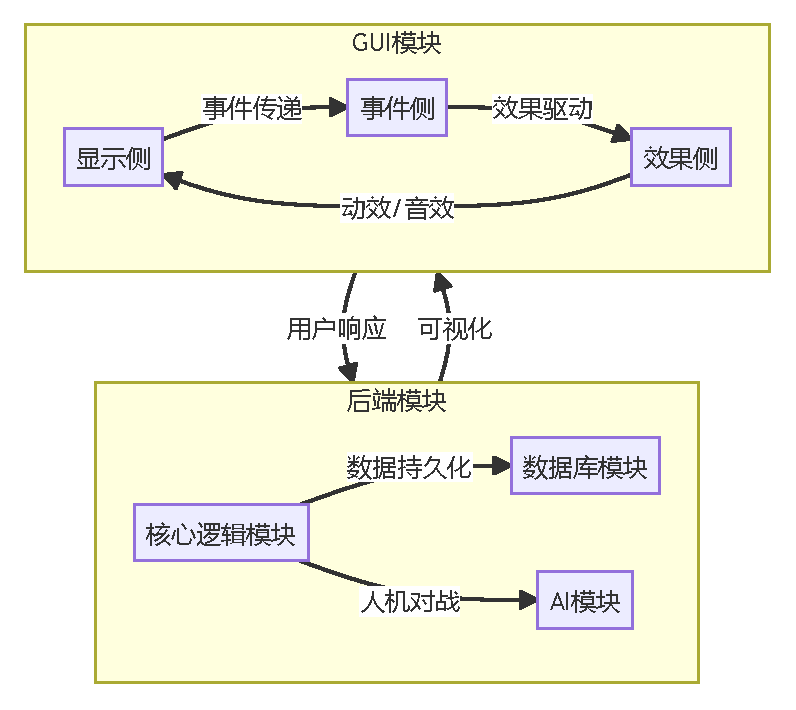
\includegraphics[width=0.6\columnwidth]{System Relationship Diagram}
\end{figure}

\subsection{详细设计}

\subsubsection{核心逻辑模块}

考虑到项目目标是实现一个简单五子棋游戏,因此对于五子棋棋局的模型抽象显得尤为重要。本项目设计\mintinline{python}{class Board},其具有以下几个主要属性以及方法:

\begin{table}[H]
    \centering
    \begin{tblr}{
            width = .6\columnwidth,
            cells ={l,m}
        }
        \toprule
        参数/方法名                                                                     & 含义       \\
        \midrule
        \mintinline{python}{timestamp}                                             & 执黑/白方玩家名 \\
        \mintinline{python}{competitor_black}/\mintinline{python}{ompetitor_white} & 执黑/白方玩家名 \\
        \mintinline{python}{board_size}                                            & 棋盘尺寸     \\
        \mintinline{python}{current_side}                                          & 执子侧      \\
        \mintinline{python}{winner}                                                & 胜利侧      \\
        \mintinline{python}{kifu}                                                  & 棋谱       \\
        \midrule
        \mintinline{python}{place(column, row)}                                    & 落子       \\
        \mintinline{python}{cancel()}                                              & 悔棋       \\
        \bottomrule
    \end{tblr}
\end{table}

核心逻辑模块有效实现了棋局状态的表示以及转移,并进行操作合法性检查,为项目其他模块的运行提供了基础。

\subsubsection{数据库模块}

如前文所述,考虑到五子棋对局数据自身结构性强,增删改查规范,使用SQLite进行数据存储其可用性要明显高于直接进行二进制文件读写。下表为数据库各列名称以及数据类型:

\begin{table}[H]
    \centering
    \begin{tblr}{
            width = .6\columnwidth,
            cells ={l,m}
        }
        \toprule
        列名                & 数据类型               \\
        \midrule
        timestamp\_       & TEXT (PRIMARY KEY) \\
        competitor\_black & TEXT               \\
        competitor\_white & TEXT               \\
        board\_size       & BLOB (NOT NULL)    \\
        kifu              & BLOB (NOT NULL)    \\
        winner            & INTEGER            \\
        \bottomrule
    \end{tblr}
    \caption{board\_table}
\end{table}

本项目设计\mintinline{python}{class BoardDatabase},其具有以下几个方法:

\begin{table}[H]
    \centering
    \begin{tblr}{
            width = .6\columnwidth,
            cells ={l,m}
        }
        \toprule
        方法名                                           & 含义           \\
        \midrule
        \mintinline{python}{append(board_to_save) }   & 增加棋局记录       \\
        \mintinline{python}{export()                } & 列出数据库中全部棋局记录 \\
        \mintinline{python}{erase(board_timestamp) }  & 删除指定棋局记录     \\
        \bottomrule
    \end{tblr}
\end{table}

\subsubsection{GUI模块}

关于显示方向,本项目设计\mintinline{python}{class Widget}以及继承子类,如下图所示:

\begin{figure}[H]
    \centering
    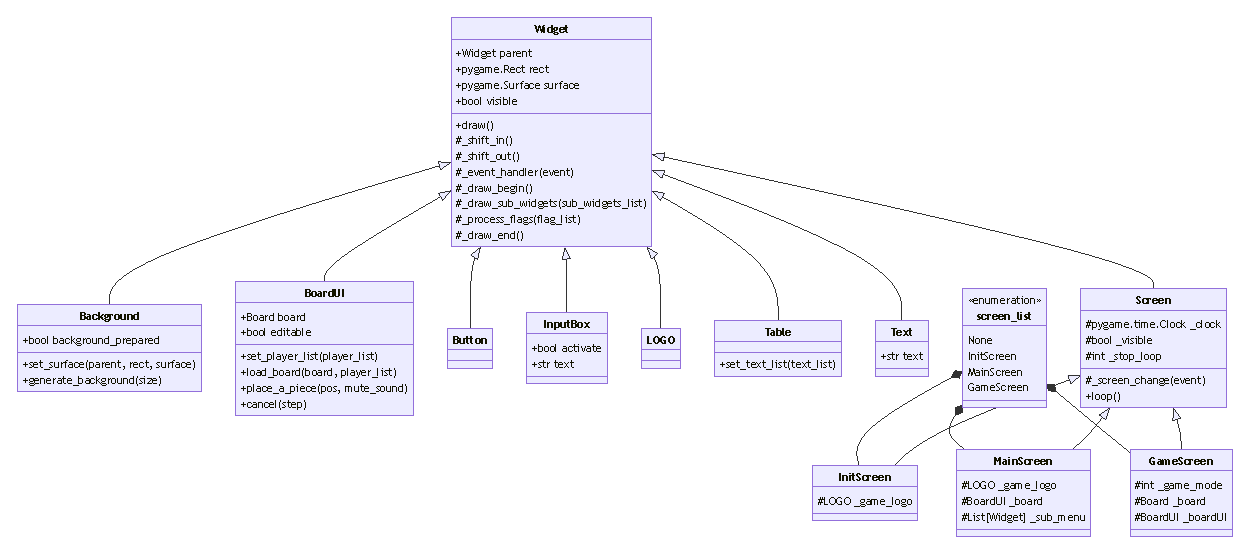
\includegraphics[width=\columnwidth]{GUI Widget Class Diagram}
\end{figure}

关于事件方向,本项目设计\mintinline{python}{_handlers[event]=function}机制,在\mintinline{python}{Screen}类执行\texttt{loop()}循环时自动提取游戏全部事件并向下层\mintinline{python}{Widget}传播,而各层\mintinline{python}{Widget}在接受事件并处理后会自动尝试向下层传播。

关于效果方向,本项目设计\mintinline{python}{class Flag}机制,用于每帧计算画面变化内容并作用到\mintinline{python}{Widget}上,其子类如下图所示:

\begin{figure}[H]
    \centering
    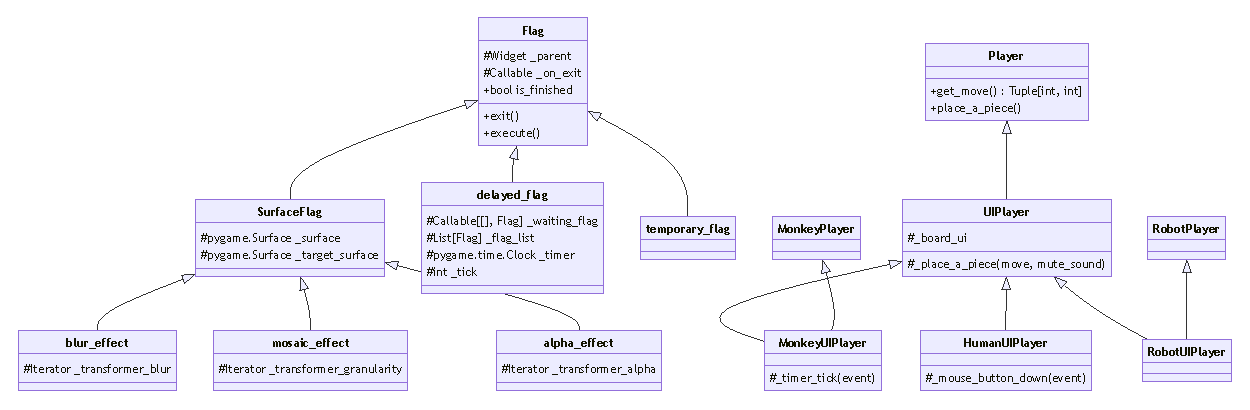
\includegraphics[width=\columnwidth]{GUI Flag and Player Class Diagram}
\end{figure}

\paragraph{注:}由于python语言自身特性,项目设计类数量较多、结构复杂(如闭包、嵌套类等),部分细节并未在上述两张图中给出。

\subsubsection{AI模块}

考虑到神经网络等智能算法对于计算机性能要求较高,而五子棋采用优化后的Min-Max搜索即可达到足够高的棋力,因此本项目最终决定参考第三方Github项目\href{https://github.com/lihongxun945/gobang}{lihongxun945/gobang},基于Python再次实现其功能。

\section{项目实现}

以下为项目实际截图:

\begin{multicols}{3}
    \begin{center}
        \foreach \x in {0,1,...,8}{
                \includegraphics[width=\columnwidth]{example/example\x}
            }
    \end{center}
\end{multicols}

截止本文档完成时,本项目为v0.2.1版本。项目源代码以及预编译二进制文件可以从\href{https://github.com/JesseSenior/pyGobang}{JesseSenior/pyGobang}获得,同时可以从\href{https://www.bilibili.com/video/BV1iL4y1N79m}{Bilibili}观看本项目v0.1.1版本的演示视频。

\section{项目目标完成情况}

\begin{todolist}
    \item[\done] 实现五子棋人人对战、人机对战;
    \item[\done] 支持对战历史记录显示、复盘、删除,支持对战信息统计;
    \item[\done] 充分应用面向对象思维,合理应用类、对象、封装、继承、多态等特性;
    \begin{todolist}
        \item[\done] 类的数量应不少于5;
        \item[\done] 继承层次结构的数量应不少于2;
    \end{todolist}
    \item[\done] 界面设计精美,交互设计友好;
    \item[\done] 支持随机文件处理(读、写、改);
    \item[\done] 源代码总行数不少于2000。
\end{todolist}

\subsection{源代码总行数统计结果}

\begin{minted}{shell}
     LINES | FILE
-----------|--------------------
        28 | ./pyGobang.py
       239 | ./src/ai.py
       103 | ./src/constants.py  
       223 | ./src/core.py
       117 | ./src/database.py
        51 | ./src/main.py
        79 | ./src/players.py
         0 | ./src/__init__.py
       205 | ./display/effect.py
       175 | ./display/texture.py
        57 | ./display/tool.py
         0 | ./display/__init__.py
       575 | ./screen/game_screen.py
       135 | ./screen/init_screen.py
       665 | ./screen/main_screen.py
        99 | ./screen/__init__.py
       138 | ./widget/background.py
       459 | ./widget/board.py
       174 | ./widget/button.py
       349 | ./widget/input_box.py
       116 | ./widget/logo.py
       282 | ./widget/table.py
        90 | ./widget/text.py
       191 | ./widget/__init__.py
       115 | ./test/core_test.py
        67 | ./test/database_test.py
         0 | ./test/__init__.py
Total Lines: 4732
\end{minted}

\end{document}